L’iridologia è una pratica pseudoscientifica di diagnosi basata sull’osservazione dell’iride.  È considerata una medicina alternativa in quanto non esiste alcun riscontro medico/scientifico che convalidi le sue teorie.  Secondo l’iridologia, l’iride è divisa in specifiche sezioni che corrispondono a specifiche parti del corpo. Le immagini seguenti rappresentano la mappa delle zone d’interesse creata dal Dr. Bernard Jensen, uno dei pionieri della teoria.

\begin{figure}[h]
  \centering
  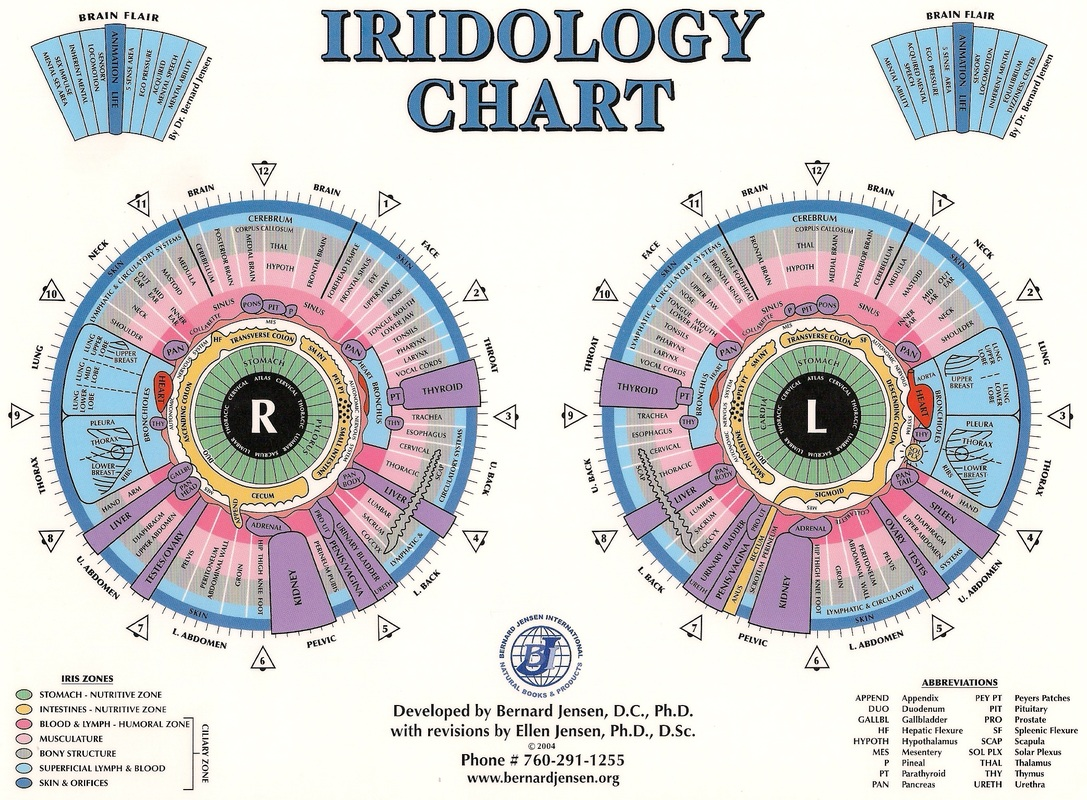
\includegraphics[scale=0.7]{iridology_chart}
  \caption{Mappa dell'iride del Dr. Bernard Jensen}
\end{figure}

Nella mappa sono state individuate 166 aree di cui 80 nell’iride destra e 86 in quella sinistra. Gli iridologi sostengono che guardando una particolare sezione dell’iride, in accordo alla mappa sopracitata, si può determinare, anche in assenza di sintomi, l’esistenza o meno di un problema nella regione del corpo relativa al segmento in esame; tuttavia la teoria non definisce quale sia la presunta malattia. Nella pratica gli iridologi generalmente usano strumenti come microscopi o lenti di ingrandimento per verificare cambiamenti nell’iride, in particolare si cercano specifici pattern di colori o irregolarità nel tessuto dell’occhio. I risultati sono poi comparati con la mappa per correlare le zone affette ai relativi organi. Quindi tutto ciò significa che un’eventuale malattia si dovrebbe riflettere in un evidente cambiamento in qualche sezione dell’iride. Molti studi tuttavia hanno dimostrato che non c’è diretta correlazione tra malattia e iride ed è per questo che la maggior parte dei dottori rigetta questa teoria. 
